% -------- Frame 1 ------
\begin{frame}{Kubernetes}
\begin{figure}
    \centering
    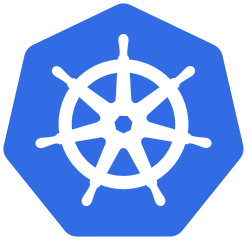
\includegraphics[width=0.2\linewidth]{static/Kubernetes_logo_without_workmark.svg.png}
\end{figure}
 The development was started by Google in 2014, but is now developed by Cloud Native Computing Foundation. 
It is the most widely used container orchestrator.

\end{frame}

% -------- Frame 2 ------
\begin{frame}{Kubernetes: Architecture}

\begin{figure}
    \centering
    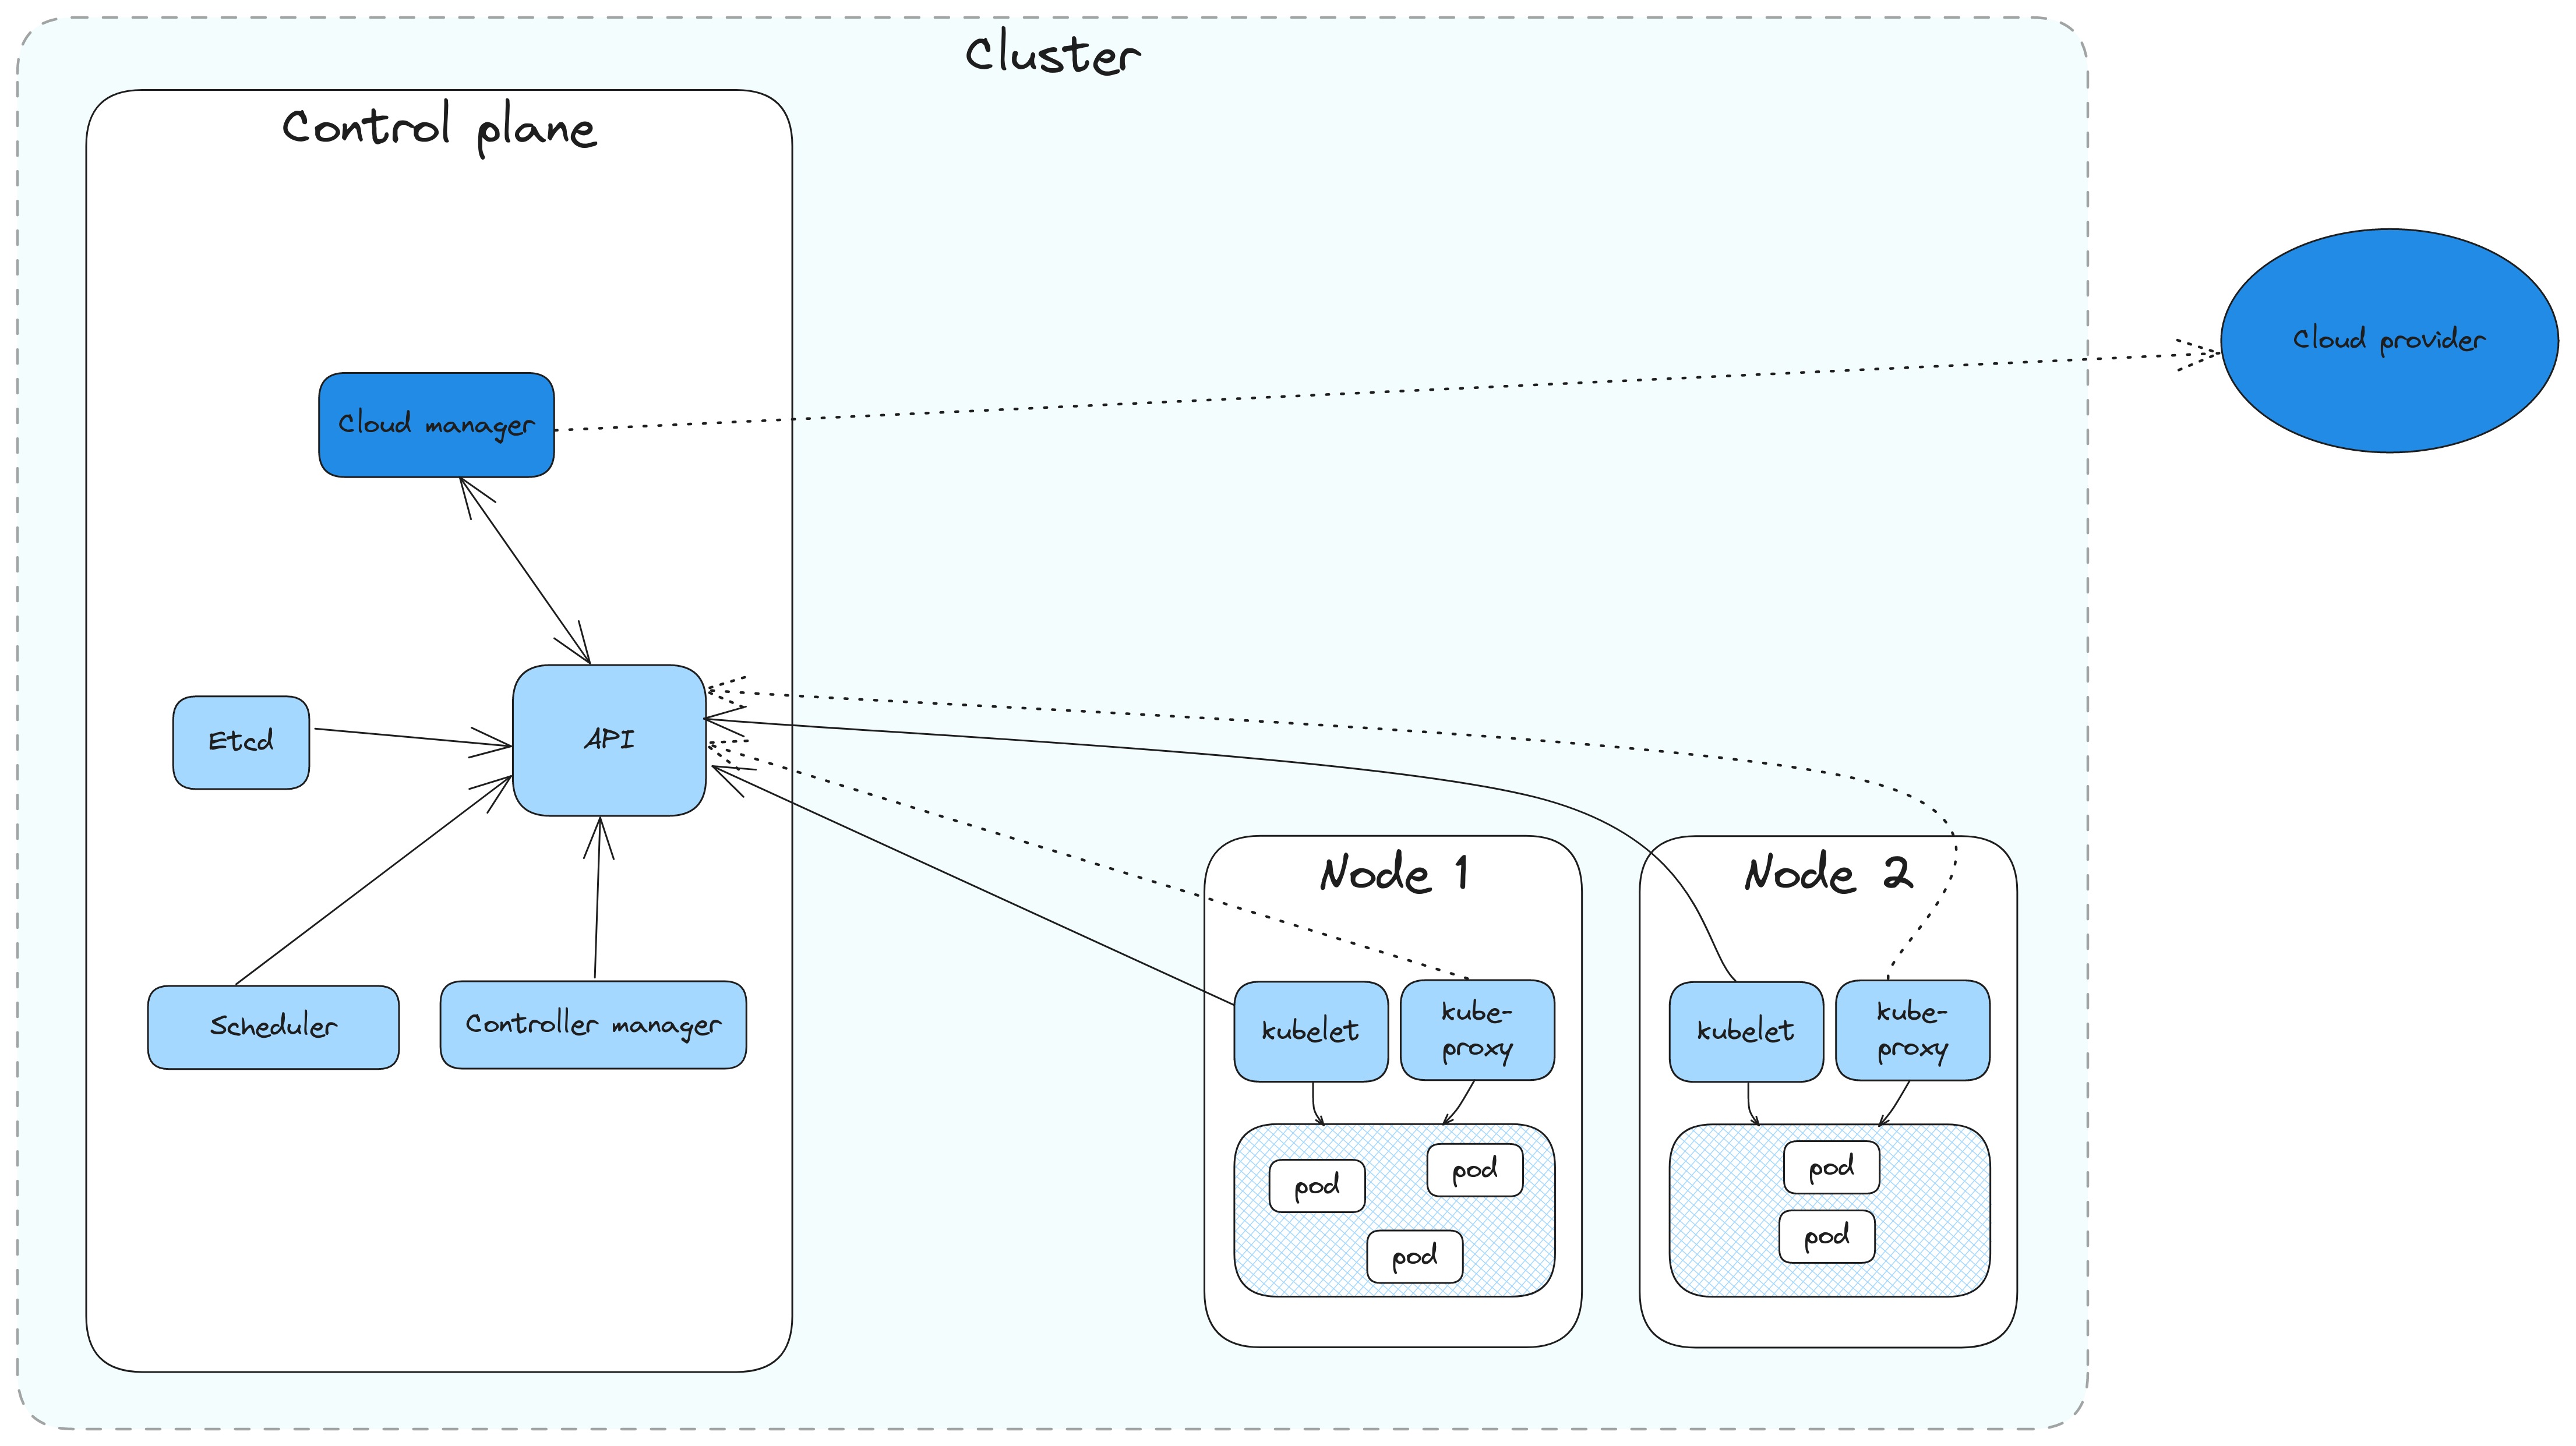
\includegraphics[width=1\linewidth]{static/Untitled-2023-09-27-1503(3).png}
\end{figure}

\begin{itemize}
    \item<2-> Something a bit less complex?
\end{itemize}

\end{frame}

% -------- Frame 3 ------
\begin{frame}{Kubernetes: Distributions}

There are a lot of distributions of K8s such as:

\begin{itemize}
    \item Kubespray \uncover<2->{\alert{\textit{It uses a set of Ansible playbooks}}}
    \item K3s \uncover<3->{\alert{\textit{Lightweight packaged as a single binary}}}
    \item MicroK8s \uncover<4->{\alert{\textit{It works on any GNU/Linux distributions using Snap package manager}}}
\end{itemize}

\end{frame}
